\chapter{Annotation \& Weighting}
\label{chap:annotation}

Using the dataset introduced in Chapter~\ref{chap:data}, this chapter focuses on adding annotation to allow for content analysis. I begin with a discussion of the development and implementation of an annotation scheme that captures aspects of native-likeness and accuracy in the picture description task (PDT) responses. In Section~\ref{sec:agreement}, I examine inter-annotator agreement for the individual annotation features on a sample of the responses, and in Sections~\ref{sec:est-feat-weights} and~\ref{sec:holistic-scoring}, I discuss how weights are assigned to these binary features in order to determine a holistic score for each response.

\section{Annotation Scheme}
\label{sec:scheme}
The goal of the annotation is to provide information that would be useful for the automatic content assessment of NNS responses via comparison with NS responses, with particular concern given to effective communication (including lexical semantics and pragmatic appropriateness) over form. The idea here is that annotations of relevant features can be used to score and then rank responses. Because my automatic assessment system relies only on surface-level features (not annotations), the system's performance can be tuned and evaluated by comparing its ranked output to the annotation-based benchmark rankings.
%A five-dimension annotation scheme was developed to capture different facets of assessment.
%
%; insights gained from the annotation, and in particular an interannotator agreement study, are covered in section~\ref{sec:agreement}.


A hypothetical ICALL system following my approach would crowdsource NS responses and use those to evaluate NNS responses, but of course such responses would not be annotated. Thus, by annotating the NS data collected in the current work, I can assess the suitability of crowdsourced NS responses for the purpose of evaluating NNS responses. \lk{addressing DS' re: what the features define in ling terms; i.e., I'm not making theoretical ling claims, i'm investigating practical process.} Indeed, the annotation features discussed in this chapter are not intended to make specific claims about NNSs' acquisition, but rather are intended to capture common ways in which a response may deviate from what is desirable in the context of the PDT at hand. These annotation features are necessary to evaluate the possibility of my broader approach of dependency-based NNS models for determining the course of a communicative ICALL activity; they are not strictly aligned with any theoretical linguistic features.

The annotation scheme was developed through an iterative process of annotation, discussion and revision, with input from two annotators and other language professionals. The annotation was developed on and applied to both NS and NNS responses. To avoid any potential bias, responses were presented to annotators in random order and without any demographic information.

In an ICALL scenario, such annotation could be used to gauge a participant's understanding, formulate feedback, and influence the next steps in the activity. This assumes that the annotations could be reliably inferred automatically, however, as manual annotation is costly and slow. In my current work, the annotations function as benchmarks which can be compared to scores provided by my automatic system, allowing for evaluation of the system itself (See Section~\ref{sec:est-feat-weights}). Furthermore, the annotation lends insights into which aspects of a response are the most difficult to account for in my approach to content assessment (and perhaps other approaches as well).

\begin{figure}[htb!]
%\begin{table}[t!] This line is giving me trouble when I go to typeset
\begin{center}
\begin{tabular}{|l|}
\hline
\multicolumn{1}{|c|}{
\includegraphics[width=0.45\columnwidth]{figures/I29.jpg}} \\
\hline
1. Holding a puppy and looks happy \\
\hline
2. She is happy with the dog. \\
\hline
3. She is wear a blue dress. \\
%3. The lady loves her dog. \\
\hline
4. hugging her dog Fluffy that she missed while on vacation. \\
\hline
5. The dog is so happy! \\
\hline
6. She loves her pet \\
\hline
\end{tabular}
\caption{\label{fig:sample-responses} Sample responses for the targeted item, \textit{What is the woman doing?}}
\end{center}
\end{figure}

The scheme was initially envisioned as a single three-point scale, ranging from \textit{accurate and native-like} to \textit{accurate but not native-like} to \textit{not accurate}---somewhat like that seen in c-rater and ensuing ETS work (see Section~
\ref{section:c-rater}, and \citealp[][]{leacock:chodorow:03,somasundaran:chodorow:14}).
This proved problematic, however, as \textit{accuracy} and \textit{native-likeness} could not be adequately defined and applied to the data as a single score.
For example, in Figure~\ref{fig:sample-responses}, it is not clear how native-like \textit{She is happy with the dog} is.  Grammatically, it is native-like, but it does not seem like an appropriate answer to the question, \textit{What is the woman doing?} Moreover, \textit{The dog is so happy!} may be native-like in terms of language use, but does not seem appropriate in the context of the question. Thus, for the purpose of analyzing content in PDT responses, native-likeness seems to encompass considerations beyond language use and grammar (i.e., broader assessment issues). 

Likewise, accuracy could not be satisfactorily defined as a simple \textit{yes} or \textit{no} construct. To illustrate, consider the ramifications of the response \textit{hugging her dog Fluffy that she missed while on vacation} (Figure~\ref{fig:sample-responses}) as either a NS or NNS response. The response does capture the main action of the item, but embellishes with unknowable details like the dog's name and the subject's motivation. This kind of response is undesirable in its own right, but would also lead to problems during the automatic scoring. If included in a set of NS responses which serve as the basis for scoring new NNS responses, this kind of embellishment would dilute the most salient and desirable information in the NS set. Furthermore, if such a NNS response is annotated as accurate, this additional information is unlikely to be readily mapped to information found in the NS set, which would lead to lower scores for the response. Accuracy, then, is an inadequate construct for the approach to content assessment envisioned for this work. Clearly, accurately capturing the main action is crucial, but \textit{verifiability} is an important consideration, as well.

In order to handle issues like those discussed above, five binary features were developed, with each feature having some relation to the original concepts of accuracy and native-likeness; a brief description of each is given below. 


\begin{enumerate}
\item \textbf{\feat{Core Event}}: Does the response capture the core event depicted in the image? Core events are not pre-defined for annotators but should be clear given the stripped down nature of the images. Crucially, the response should link an appropriate subject to the event.  In Figure~\ref{fig:sample-responses}, \textit{[The woman is] holding a puppy and looks happy} clearly captures the core event, while \textit{She is wear a blue dress} is irrelevant to the event happening.
\item \textbf{\feat{Answerhood}}: Does the response make a clear attempt to answer the prompt question? This generally requires a progressive verb, because the PDT questions are in the present progressive. For targeted items, the subject of the question or an appropriate pronoun must be used as the subject of the response.  For example, \textit{The dog is so happy!} (Figure~\ref{fig:sample-responses}) is answering a question other than \textit{What is the woman doing?}. 
\item \textbf{\feat{Grammaticality}}: Is the response free from errors of spelling and grammar?  
This is a relatively straightforward feature to annotate. For example, from Figure~\ref{fig:sample-responses}, \textit{She is wear a blue dress} contains an ungrammatical verb form.
\item \textbf{\feat{Interpretability}}: Does the response evoke a clear mental image (even if different from the actual item image)? Any required verb arguments must be present and unambiguous.  For example, \textit{She loves her pet} (Figure~\ref{fig:sample-responses}) is too vague to generate a clear mental image. No action is specified (unless we force an unlikely reading of \textit{loves} as a dynamic, simple present verb), and we cannot know if the \textit{pet} is a dog, a goldfish, etc.
\item \textbf{\feat{Verifiability}}: Does the response contain only information that is true and verifiable based on the image? Inferences should not be speculations and are allowed only when necessary and highly probable, as when describing a familial or professional relationship between persons depicted in the image.  For example, in Figure~\ref{fig:sample-responses}, \textit{She is wear a blue dress} conveys information that is irrelevant to the core event but is nonetheless recoverable from the image (\feat{core event}=0, \feat{verifiability}=1), while \textit{hugging her dog Fluffy that she missed while on vacation} fulfills the core event but also has information that cannot be verified from the picture (\feat{core event}=1, \feat{verifiability}=0).
\end{enumerate}











These features, as mentioned above, were developed in direct response to concerns encountered when trying to apply the constructs of \textit{accuracy} and \textit{native-likeness} to the PDT responses. \feat{Verifiability}, for ensuring that the response information is indeed in the image, emerged from scenarios like the one where a participant gave the name \textit{Fluffy} to the unnamed dog in the prompt in Figure~\ref{fig:sample-responses}. \feat{Answerhood} was included to address responses that do not offer an answer to the PDT question, even when the topic of the response is on-target. \feat{Grammaticality} was deemed necessary, as it would be helpful for even a semantics-focused feedback module to know if a response is grammatically well-formed. These three features were the least difficult to operationalize (and indeed resulted in the highest inter-annotator agreement scores, as shown in Section~\ref{sec:agreement}).

The other two features, which came to be labeled \feat{Core event} and \feat{interpretability}, took more effort and iteration to define. In existing ICALL research, discussions of annotation for learner productions are almost exclusively focused on syntactic forms and errors, and precedent for operationalizing more semantic features is lacking. \feat{Core event} was somewhat inspired by the ``lexical core'' concept presented by \citet{bardovi2017unconventional}; in a study of second language learners' acquisition of formulaic language, the researchers identified the minimal portion of a conventional expression necessary for conveying that expression, as determined by a majority usage among NSs. \feat{Core event} is not determined by majority NS usage, as the PDT is not intended to elicit specific forms acquired as conventional expressions. It does, however, attempt to label responses that contain the minimal elements required for conveying the PDT actions---the linking of an appropriate verb and any syntactically and semantically required objects. \feat{Interpretability}, as intended here, is largely unconcerned with the particulars of syntactic structures, but nonetheless found relevant precedent in research regarding multi-layered syntactic annotation, like \citet{ragheb2014developing}, where uninterpretable elements that may prevent analysis on other layers are flagged as \textit{unknown}. \feat{Interpretability} (operationalized here as whether or not the sentence can evoke a clear mental image, see below) is not necessarily indicative of the other features, but it would certainly be useful for a feedback module (as would \feat{grammaticality}).

As with most annotation schemes in linguistics, the final SAILS scheme is a compromise. This scheme represents the minimal set of features necessary to accomplish two major goals of this work: investigating the use of NS responses as an evaluation model for NNS, and examining the factors that lead a NNS response to be rated highly or lowly. Besides the features explained below, others were explored but rejected. For example, a \textit{good faith} feature was considered to identify responses that were not given in good faith, such as gibberish, profanity and irrelevant responses. Such a discrimination was applicable to less than three percent of responses in the sample used for developing the annotation scheme, however, so this feature was deemed too costly for the value it would provide. Moreover, this feature is largely subsumed by the others, as bad faith responses tend to score poorly across the board.

A set of annotation guidelines was produced with definitions, rules and examples for each feature. For most features, the rules for targeted and untargeted items (see Section~\ref{sec:pdt}) vary slightly; the untargeted rules are generally less strict to accommodate the less restrictive prompt question. The complete annotation guide is included in Appendix~\ref{appendix:annotation_guide}.
%The features and brief descriptions are listed here and discussed further in the discussion of inter-annotator agreement in Section~\ref{sec:agreement}.

\begin{figure}[htb!]
%\begin{table}[t!] This line is giving me trouble when I go to typeset
\begin{center}
\begin{tabular}{c}
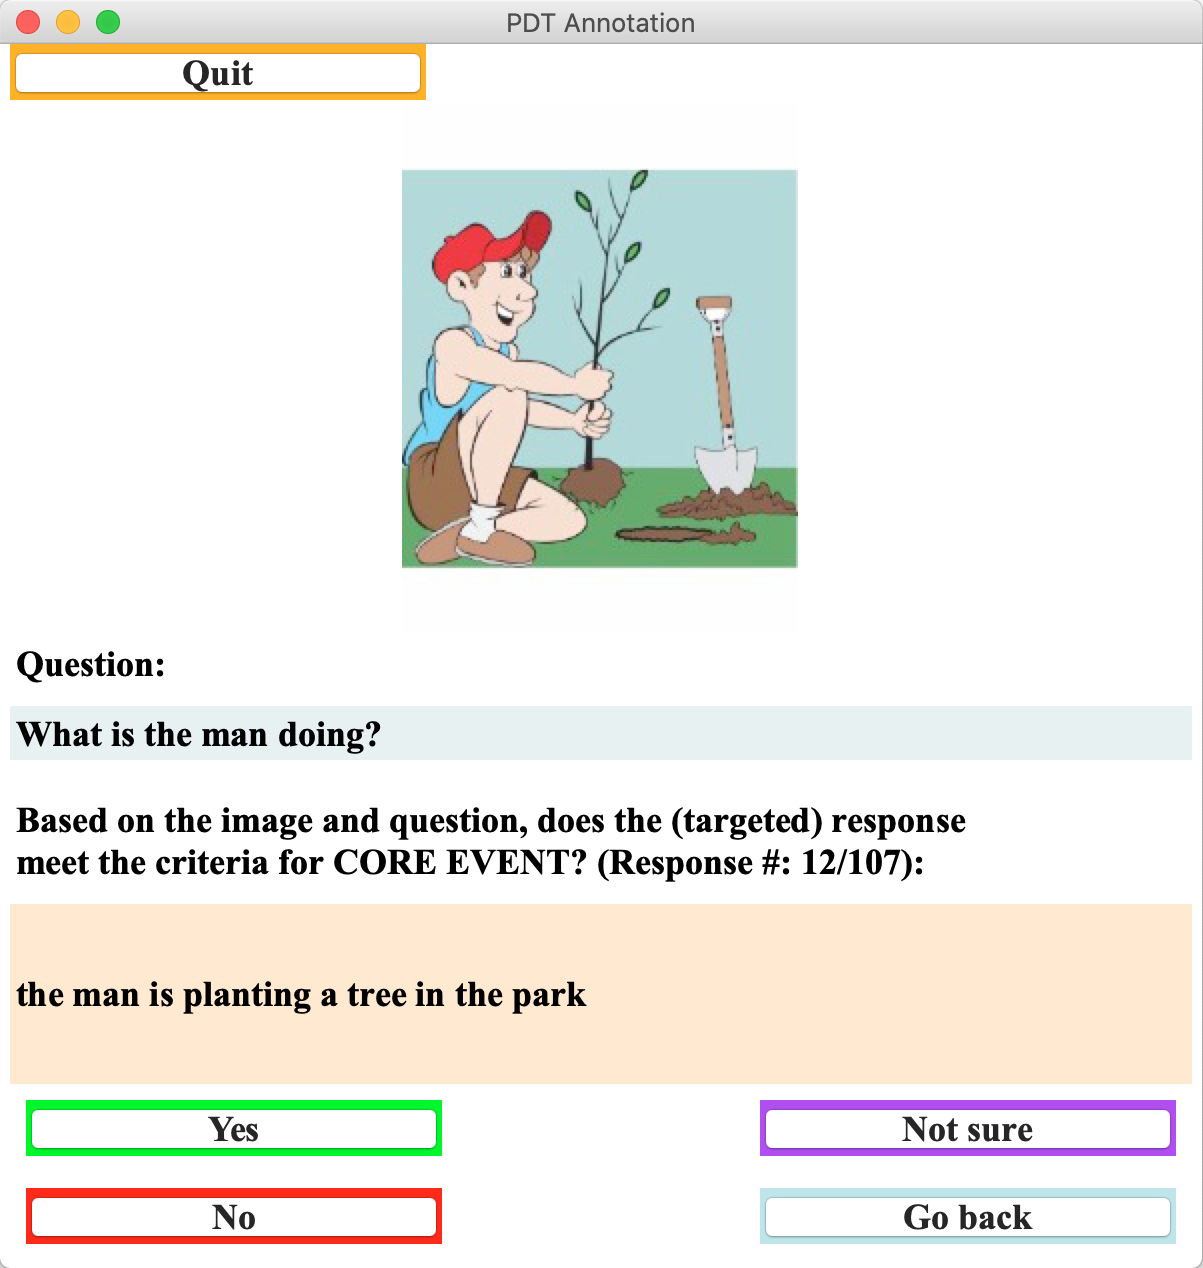
\includegraphics[width=0.85\columnwidth]{figures/annotation_interface.jpg} \\
\end{tabular}
\caption{\label{fig:annotation-interface} Interface used for feature annotations. Note that ``Not sure'' is not a final annotation value; it merely moves the response to the end of the queue.}
\end{center}
\end{figure}



\paragraph{Annotation process}
The annotation was performed one feature at a time, so that annotators did not have to remember the criteria for multiple features while working through the responses. To facilitate this workflow, I created a simple interface that displays the PDT image and question, along with the current feature name and prompt for the annotator, shown in Figure~\ref{fig:annotation-interface}. The interface writes these annotations to a spreadsheet.

\begin{table}[htb!]
%\begin{table}[t!] This line is giving me trouble when I go to typeset
\begin{center}
%\begin{tabular}{|p{3.7cm}|c|c|c|c|c|}
\begin{tabular}{|l|c|c|c|c|c|}
\hline
%\multicolumn{6}{|c|}{
\includegraphics[width=0.45\columnwidth]{figures/I02.jpg}} \\
\multicolumn{6}{|c|}{
\includegraphics[width=0.45\columnwidth]{figures/I02.jpg}} \\
\hline
%\multicolumn{3}{|l|}{What is the woman doing? [Intransitive]} \\
\textit{What is the boy doing?} & C & A & G & I & V \\
\hline
\hline
He is eating food. & 0 & 1 & 1 & 1 & 1 \\
\hline
eatting. & 0 & 1 & 0 & 1 & 1 \\
\hline
The child is about to eat pizza. & 1 & 0 & 1 & 1 & 1 \\
\hline
He may get fat eating pizza. & 1 & 0 & 1 & 1 & 0 \\
\hline
\hline
\hline
\textit{What is happening?} & C & A & G & I & V \\
\hline
\hline
Child is eating pizza. & 1 & 1 & 0 & 1 & 1 \\
\hline
Tommy is eating pizza. & 1 & 1 & 1 & 1 & 0 \\
\hline
The boy's eating his favorite food. & 0 & 1 & 1 & 0 & 0 \\
\hline
Pizza is this boy's favorite food. & 0 & 0 & 1 & 0 & 0 \\
\hline
\end{tabular}
\caption{\label{tab:dev-transitive} Targeted and untargeted sample responses from the development set transitive item, shown with adjudicated annotations for \feat{core event} (\textit{C}), \feat{answerhood} (\textit{A}), \feat{grammaticality} (\textit{G}), \feat{interpretability} (\textit{I}) and \feat{verifiability} (\textit{V}).}
\end{center}
\end{table}



\paragraph{Example annotations}

Table~\ref{tab:dev-transitive} presents example responses with all five features annotated, illustrating each feature's distinctiveness from the others.  For example, for \textit{He is eating food} one can generate a mental picture, e.g., of someone chewing (\feat{in\-ter\-pret\-a\-bil\-i\-ty}=1), but the pizza is important to the item image (\feat{core event}=0).  As another example, \textit{He may get fat eating pizza} seems to be addressing a question about the consequences of the eating action rather than the actual prompt question (\feat{answerhood}=0). Moreover, the response talks about hypotheticals not in the picture (\feat{verifiability}=0).
%, while all other features are correct.  
Teasing apart these annotations and their reliability between annotators is the focus of the next section.


\section{Agreement}
\label{sec:agreement}
Two annotators participated in the annotation. Both are native speakers of (US) English, and each had several years of language teaching experience with both children and adult learners at the time. Annotator 1 (A1) annotated the complete corpus. Annotator 2 (A2) annotated only the working set and the agreement assessment set, data subsets described next.

Three items were used as a working set for creating and revising the annotation scheme. These items were also used as examples in the final version of the guidelines. They represent one intransitive, one transitive and one ditransitive event. Both annotators annotated portions of the working set multiple times throughout the process, discussing and adjudicating disagreeing annotations before moving on to the agreement assessment set, which was completed without consultation between the annotators.

%% LK NTS:
%%intransitive is I30 (woman is running)
%%transitive is I29 (woman is hugging dog)
%%ditransitive is I28 (man is giving directions)
\begin{figure}[htb!]
%\begin{table}[t!] This line is giving me trouble when I go to typeset
\begin{center}
\begin{tabular}{|c|c|c|}
\hline
{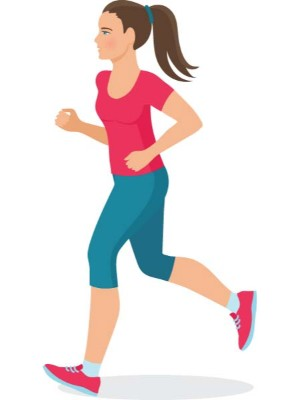
\includegraphics[width=0.29\columnwidth]{figures/I30.jpg}} & {
\includegraphics[width=0.3\columnwidth]{figures/I29.jpg}} & {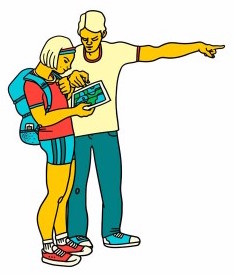
\includegraphics[width=0.3\columnwidth]{figures/I28.jpg}} \\
\hline
What is the woman doing? & What is the woman doing? & What is the man doing? \\
\hline
\end{tabular}
\caption{\label{fig:test-sample-items} The targeted PDT items used for assessing inter-annotator agreement. In the untargeted form, the question for each is \textit{What is happening?} From left to right, these examples represent one canonically intransitive, one transitive, and one ditransitive item.}
\end{center}
\end{figure}

The agreement assessment set parallels the working set and consists of one intransitive, one transitive, and one ditransitive item; it is shown in Figure~\ref{fig:test-sample-items}. Agreement and Cohen's kappa scores are given in Table~\ref{tab:agreement}, broken down by different criteria.  The following sections will examine the results, comparing verb types (transitivity), targeted and untargeted items, the five features, and NS and NNS participants.

\begin{table*}[htb!]
\begin{center}
\begin{tabular}{|l|l|l|l|l||l|l||l|}
\hline
Set	& Total	& A1Yes & A2Yes & AvgYes & Chance & Observ & Kappa \\
\hline
\hline
Intransitive & 2155 & 0.863 & 0.855 & 0.859 & 0.758 & 0.978 & 0.910 \\
\hline
Transitive & 2155 & 0.780 & 0.774 & 0.777 & 0.653 & 0.949 & 0.853 \\
\hline
Ditransitive & 2155 & 0.812 & 0.786 & 0.799 & 0.678 & 0.924 & 0.764 \\ 
\hline
\hline
Targeted & 3390 & 0.829 & 0.818 & 0.824 & 0.709 & 0.949 & 0.823 \\
\hline
Untargeted & 3075 & 0.806 & 0.790 & 0.798 & 0.678 & 0.952 & 0.872 \\
\hline
\hline
\feat{Core Event} & 1293 & 0.733 & 0.717 & 0.725 & 0.601 & 0.923 & 0.808 \\
\hline
\feat{Answerhood} & 1293 & 0.834 & 0.831 & 0.833 & 0.721 & 0.982 & 0.936 \\
\hline
\feat{Grammaticality} & 1293 & 0.861 & 0.872 & 0.866 & 0.768 & 0.960 & 0.827 \\
\hline
\feat{Interpretability} & 1293 & 0.818 & 0.787 & 0.802 & 0.682 & 0.919 & 0.744 \\
\hline
\feat{Verifiability} & 1293 & 0.845 & 0.817 & 0.831 & 0.719 & 0.968 & 0.884 \\
\hline
\end{tabular}
\caption{\label{tab:agreement} Agreement scores broken down by different properties of the agreement assessment set: total annotations (\textit{Total}), \textit{yes} annotations for Annotator 1 and 2 (\textit{A1Yes}, \textit{A2Yes}), average \textit{yes} annotations (\textit{AvgYes}), total expected chance agreement for \textit{yes}es and \textit{no}s (\textit{Chance}), actual observed agreement (\textit{Observ}) and Cohen's kappa (\textit{Kappa}).}
\end{center}
\end{table*}

\subsection{Transitivity} 
\label{sec:transitivity}
Comparing the intransitive, transitive, and ditransitive items revealed an association between agreement and item complexity. The highest raw agreement and Cohen's kappa scores were found with the intransitive item ($97.8\%$, $\kappa=0.910$) and the lowest with the ditransitive ($92.4\%$, $\kappa=0.764$). 

This was as expected, as ditransitive sentences are longer and have more verbal arguments, making for more opportunities for responses to vary (see Table~\ref{tab:ttr}), and thus more opportunities for annotators to disagree on a response. This trend also matched annotator feedback: in a follow-up consultation, both noted the ditransitive item as the most difficult to annotate overall, and the intransitive as the easiest.

\subsection{Targeting} 
\label{sec:prompts}
Across the targeting parameter, the raw agreement scores were comparable ($94.9\%$ for targeted and $95.2\%$ for untargeted items). However, the untargeted group had a higher kappa score ($0.823$ for targeted items versus $0.872$ for untargeted items).

When asked to compare the annotation process for targeted and untargeted items, A1 suggested that problems are easier to identify in untargeted item responses because the setting is more relaxed and may allow for responses that deviate noticeably from the desired content. A2 noted that targeted responses require more concentration and closer consultation of the guidelines. For example, \feat{answerhood} does not allow for targeted responses to modify the subject provided in the question in any way, whereas in answering \textit{What is happening?}, the respondent is free to speak of characters in the pictures in many different ways.  Both A1 and A2 thus described the annotation of untargeted items as less restrictive and less time-consuming.

\subsection{Features} 
\label{sec:features}
Grouped by feature, the annotations all showed raw agreement scores above 91\% and Cohen's kappa scores above 0.74 (Table~\ref{tab:agreement}). For future use of this corpus in content assessment, these kappa scores are comfortably above the 0.67 suggested as a threshhold for meaningful, reliable agreement \citep{landis1977measurement, artstein:massimo:2008}.  I discuss each feature in turn here, highlighting difficulties in coming to an agreement, as such disagreements illustrate some of the impactful ways in which responses vary.

\paragraph{\feat{Core event}} Isolating whether the main content of the picture is described in the response, the \feat{core event} feature is the most relevant of the five for content assessment. All five features were skewed toward \textit{yes} annotations, but with an average \textit{yes} rate of 72.5\%, core event was the least skewed; i.e., more responses received a \textit{no} annotation for \feat{core event} than for any other feature.

\feat{Core event} had the second lowest inter-annotator agreement kappa score, at 0.808. This was somewhat lower than expected, as the pre-adjudication working set score was 0.889. This appears to be largely attributable to the difficulty of the ditransitive item in the agreement assessment set, challenging for both participants and annotators (section~\ref{sec:transitivity}). 

The main issue in this case has to do with the amount of specificity required to capture the core event.  The working set ditransitive item depicts a man delivering a package to a woman, and most responses described this as such a transaction, using \textit{give}, \textit{deliver} or \textit{receive}. The agreement assessment set item shows a man giving directions to a woman (Figure~\ref{fig:test-sample-items}), and this resulted in a greater degree of variation. This is confirmed by the lower type-to-token ratio  (TTR) of main verbs among working set responses versus agreement assessment set responses (0.189 versus 0.247), as presented in Table~\ref{tab:pref-dev-vs-test}. Many  (particularly NNS) responses portrayed this not as a canonical \textit{giving directions} event but as \textit{pointing}, 
%\textit{guiding}, 
\textit{helping a lost person} or \textit{reading a map}, with A2 more likely to accept these less specific descriptions.

\begin{table}[htb!]
\begin{center}
\begin{tabular}{|l||r|r||r|r|}
\hline
 & \multicolumn{2}{|c||}{Development Set} & \multicolumn{2}{|c|}{Test Set} \\
\hline
Version	& Types/Tokens & TTR & Types/Tokens & TTR \\
\hline
\hline
NNS Target & 12/71 & 0.169 & 16/70 & 0.229 \\
\hline
NS Target & 32/157 & 0.204 & 37/156 & 0.237 \\
\hline
NNS Untarg & 14/70 & 0.200 & 18/71 & 0.254 \\
\hline
NS Untarg & 33/180 & 0.183 & 36/134 & 0.269 \\
\hline
\hline
Average & 22.8/119.5 & 0.189 & 26.8/107.8 & 0.247 \\
\hline
\end{tabular}
\caption{\label{tab:pref-dev-vs-test} Comparing type-to-token ratios (\textit{TTR}) for \textbf{main verbs} among the working set and agreement assessment set \textbf{ditransitive items}; greater variation correlates with lower \feat{core event} inter-annotator agreement, which helps explain why in Table~\ref{tab:agreement} \feat{core event} agreement is lower than agreement for other features.}
\end{center}
\end{table}

Similarly, but to a lesser extent, the transitive item, which shows a woman hugging a dog (Figure~\ref{fig:test-sample-items}), resulted in disagreements where A2 accepted the word \textit{pet} as the object, but A1 rejected such responses as too vague. Despite the acceptable scores for \feat{core event} agreement, the fact that many disagreements hinged on particular word choice or annotators having minor differences in interpretation of the event suggests that greater agreement could be achieved by providing annotators with suggestions about the acceptable content for each response. In other words: by more clearly determining the desired level of specificity of a response---for the verb or its arguments---agreement could be higher. The desired specificity may vary in accordance with the intended use of the annotations; in the current annotations, the standard discussed between annotators and in the guidelines (see Appendix~\ref{appendix:annotation_guide}) included pragmatic considerations like naturalness, native-likeness and effort.

\paragraph{\feat{Answerhood}} Capturing the semantic content of the picture is not the only criterion for determining the quality of a response; the \feat{answerhood} feature was added largely as a way to identify responses that simply do not follow the instructions. Such responses tend to fall into one of the following categories:

\begin{enumerate}
\item Responses that do not directly answer the given question, perhaps by reframing the perspective so that it seems like a different question was asked, e.g., \textit{He may get fat eating pizza}, in response to \textit{What is the boy doing?} (Table~\ref{tab:dev-transitive});
\item Responses that are gibberish or very low-effort and entered only so the participant can proceed to the next item, e.g., \textit{Hey man};
\item ``Troll'' responses that attempt to be clever (or sometimes obscene) at the cost of attempting a direct answer, e.g., \textit{How is the pizza staying perfectly horizontal when the boy is holding it so close to the tip?}, in response to \textit{What is happening?} (Table~\ref{tab:dev-transitive}).
\end{enumerate}

The majority of participants did attempt to follow the instructions and answer the question, however, and it is unsurprising that this feature skewed strongly toward \textit{yes} annotations and resulted in the highest raw agreement (98.2\%) and kappa (0.936) scores among the five features.

Of 23 disagreements, seven stemmed from one annotator failing to enforce the requirement that a targeted response subject be either an appropriate pronoun or the exact subject given in the question, without adjectives, relative clauses or other modifiers. Given the question \textit{What is \textbf{the woman} doing?}, for example, the responses \textit{The \textbf{lady} is running} and \textit{The woman \textbf{who in pink} is running} were incorrectly accepted by one annotator each.  While this criterion may seem strict, this subject-identity rule separates the problem of identifying an attempt to answer the question from the problem of verifying information (see \feat{verifiability} below).

Another ten disagreements involved responses lacking a progressive verb, generally required as an indication that the response refers to the specific action in the image and does not merely describe a state or a general truth (cf., e.g., \textit{The woman is running} vs. \textit{The woman runs}). Annotator fatigue thus appeared to account for the majority of \feat{answerhood} disagreements.
%\smallskip

\paragraph{\feat{Grammaticality}} The \feat{grammaticality} feature was the most heavily skewed one, with an average \textit{yes} rate of 86.6\%.  As the only non-semantic annotation, this was perhaps not surprising.

\feat{Grammaticality} had a raw agreement score of 96.0\% and a kappa of 0.827. Among 52 disagreements, annotators concurred in discussion that 19 involved an avoidable annotator error. These were primarily responses with typos, misspellings, subject-verb disagreement and bare nouns, all rejected by the annotation rules. Such cases are likely attributable to annotator fatigue.

% http://www.cs.rochester.edu/~tetreaul/acl11-mturk-grammar.pdf
The remainder reflect an unavoidable level of disagreement. Many of these stemmed from differing interpretations of bare nouns as either errors or as acceptable mass nouns, as in \textit{The man is giving \textbf{direction} to the tourist}. In several cases, annotators disagreed over prepositions, which are known to be a common source of disagreement and pose special challenges in the context of learner language \citep{tetreault-chodorow:2008:HJCL,tetreault:chodorow:08}. For example, annotators did not agree on the grammaticality of the prepositions in \textit{The girl is asking for help \textbf{to} the man} and \textit{The girl is hugging \textbf{with} her cat}. 

\paragraph{\feat{Interpretability}} The average \textit{yes} rate for \feat{interpretability} was 0.802; only \feat{core event} was less skewed.
%
The raw agreement score was 91.9\% and kappa is 0.744, the lowest scores among the five features. This was anticipated, because \feat{interpretability} is perhaps the most difficult to define, leaving room for annotators' personal judgments. Annotators must decide whether a given response evokes a clear mental image, regardless of how well that mental image matches the PDT image.  In this way, responses such as \textit{The man is working} which may %contain all \feat{core event} information and 
be completely \feat{verifiable} may still fall short, in that the man could be picking fruit, building a bridge, and so forth.

The guidelines place some restrictions on what it means to be a clear mental image. To begin with, if one were to illustrate the response, the result would be a complete, representational, canonical image. It would not be necessary to guess at major elements, like subjects or objects. 
%
All necessary verb arguments would be identifiable from the sentence and thus not obscured or out of the frame in the mental image.
%
Vague language should be avoided, but human gender does not need to be specified, especially when a non-gendered word like \textit{doctor} or \textit{teacher} is natural. 

Consider a response like \textit{A woman is receiving a package}.  By these criteria, the response is annotated as 0 because the person or entity delivering the package is not specified, and an illustrator would need to either guess at a depiction of the deliverer, or compose the image with the deliverer conspicuously out of the frame. \textit{A man is delivering a package}, on the other hand, would be accepted. An illustrator could simply show a delivery person carrying a package or placing it in a mailbox or on a doorstep, as an indirect object is not necessary to convey the meaning of the verb \textit{deliver}.

Among the 105 annotator disagreements, fatigue accounts for roughly 30; this was difficult to determine precisely because annotators expressed difficulty in identifying a single root cause for many disagreements. Those that were clearly attributable to annotator error tended to involve responses with some internal inconsistency, as with subject-verb disagreements, where the number of the subject was uninterpretable (e.g., \textit{The woman are hugging the dog}). Among true disagreements, the level of specificity was often the point of contention, as with \feat{core event}. For example, A1 accepted several transitive item responses with the verb \textit{love}, as in \textit{The woman loves her dog} (Figure~\ref{fig:test-sample-items}). A2 argued that these are too vague to illustrate as an action, but A1 disagreed. This disagreement may also hinge on differing judgments regarding the use of \textit{love} as a dynamic verb, and such idiolectal differences are an unavoidable source of noise in annotating this feature. As mentioned above (see \feat{verifiability} below), expanding the guidelines might help cover some such situations, but likely at the cost of increased annotator fatigue.

\paragraph{\feat{Verifiability}} On the flipside of the question of whether the core semantic content is expressed is the question of whether any extraneous content is added, or any content used in a way which cannot be verified from the picture.  The average \textit{yes} rate for \feat{verifiability} was 83.1\%, making it the third most skewed feature.

The raw agreement score was 96.8\%, and the kappa score was 0.884. By both measures, this was the second highest agreement score, after \feat{answerhood}. Of 42 disagreements for \feat{verifiability}, annotators agreed that at least eight were avoidable. Of these, five involved the incorrect use of plurals. For example, A1 accepted \textit{A man is pointing the way for the women}, when the image showed only one woman, but the guidelines reject such responses. Two other errors stemmed from inaccuracy, with respondents referring to a dog in the illustration as a cat. Each annotator incorrectly accepted one such response. One disagreement involved the misspelling of a crucial object: \textit{The woman is holding the pat}. It was unclear whether \textit{pet} or \textit{cat} was intended. This should have rendered the response unverifiable, but A1 accepted it.

The remaining disagreements are attributable to different opinions about inferences.  For the ditransitive item, for example, both annotators accepted responses that refer to the woman as a \textit{hiker}, but only A1 accepted responses where the man and woman are collectively referred to as hikers. For the intransitive item depicting a woman running, A1 accepted multiple responses that refer to this as \textit{a race}, as well as responses that inferred the runner's motivation (fitness, leisure, etc.). I believe such differences are unavoidable in this annotation task. Adding more detail to the guidelines might help reduce disagreements about inferences, but the guidelines are nearly 40 pages and expanding them to cover various contingencies would certainly add to annotator demand and fatigue.
%The rate of such disagreements might be reduced slightly by adding more detail to the annotation guidelines or having annotators calibrate their ratings with an extended set of sample items, but these increased demands on annotators might also lead to greater annotator fatigue. In other words, the current definition of the feature is a compromise.

\subsection{NS \& NNS Responses}
\label{NSandNNSagreement}
Response quality and annotation agreement were also calculated separately for NS and NNS responses, as shown in Table~\ref{tab:NSvNNSagreement}. The average rate of \textit{yes} annotations is used here as an indication of response quality. Comparing this \textit{yes} rate shows that the NNSs outperformed the NSs by between roughly 8\% and 12\% on all features except \feat{grammaticality}. It is not surprising that NSs outperformed NNSs on this feature (90.2\% to 79.3\%), but to account for their superior performance of NNSs on the other features, one must consider the fact that the NNSs were recruited from English courses and performed the task with peers and researchers present. The NNSs were more likely to make a good faith effort than the NSs, the majority of whom performed the task anonymously and remotely. Furthermore, 
%only NSs were asked to provide two responses to each item; 
with twice as many responses to provide for each item for NSs, fatigue and boredom may have been a contributing factor.
%; related task effects and fatigue are also likely contributing factors.

%% LK NTS:
%%intransitive is I30 (woman is running)
%%transitive is I29 (woman is hugging dog)
%%ditransitive is I28 (man is giving directions)

%%Set	& Total	& A1Yes & A2Yes & AvgYes & Chance & Observed & Kappa \\
\begin{table}[htb!]
\begin{center}
\begin{tabular}{|l||l|l||l|l||l|l||l|l|}
\hline
 & \multicolumn{2}{|c||}{Average Yes} & \multicolumn{2}{|c||}{Chance Agree} & \multicolumn{2}{|c||}{Observed Agree} & \multicolumn{2}{|c|}{Kappa} \\
\hline
 Set & NS & NNS & NS & NNS & NS & NNS & NS & NNS \\
\hline
\hline
\feat{Core}  & 0.686 & 0.805 & 0.569 & 0.686 & 0.922 & 0.927 & 0.819 & 0.767 \\
\hline
\feat{Answer}  & 0.800 & 0.899 & 0.680 & 0.819 & 0.977 & 0.993 & 0.928 & 0.961 \\
\hline
\feat{Gramm}  & 0.902 & 0.793 & 0.823 & 0.671 & 0.962 & 0.955 & 0.786 & 0.863 \\
\hline
\feat{Interp}  & 0.764 & 0.881 & 0.638 & 0.789 & 0.910 & 0.936 &  0.752 & 0.697 \\
\hline
\feat{Verif}  & 0.807 & 0.882 & 0.687 & 0.791 & 0.970 & 0.962 & 0.904 & 0.819 \\
\hline
\end{tabular}
\caption{\label{tab:NSvNNSagreement} Comparing feature annotation agreement scores for NSs and NNSs: average \textit{yes} annotations (\textit{Average Yes}), total expected chance agreement (for \textit{yes}es and \textit{no}s) (\textit{Chance Agree}), actual observed agreement (\textit{Observed Agree}) and Cohen's kappa (\textit{Kappa}).}
\end{center}
\end{table}

Turning to the question of annotation quality, raw agreement scores were high among both groups, ranging from 91\% to 99.3\%. Notably, for \feat{core event},  \feat{verifiability} and \feat{interpretability}, kappa scores were higher for NS responses than for NNS responses. It may be no coincidence that these three features are the most closely tied to meaning, while \feat{answerhood} gets at pragmatics and \feat{grammaticality} focuses on form.

The lower kappa score for NS \feat{answerhood} is also attributable to task effects, as a second response (as required of NSs) is more likely to be off-topic or in bad faith. For \feat{grammaticality}, kappas for annotator agreement were higher for NNS responses. A relatively low rate of expected (chance) agreement contributes to this fact. Additionally, annotators noted that many grammar problems with NNS responses were obvious (e.g., \textit{The \textbf{man who in yellow} is showing the way to a girl}, see Figure~\ref{fig:test-sample-items}), but the few grammar problems in the NS data were mostly typos and more easily overlooked (e.g., \textit{The man is giving \textbf{ditections}}).

\section{Establishing Feature Weights}
\label{sec:est-feat-weights}

The five annotation features were chosen for their relevance to the construct of overall ``response goodness'' for the picture description task (PDT). However, we cannot assume that these binary features bear equal weight in determining the quality of a response. Certainly \feat{core event} is more important than \feat{grammaticality}, for example. Thus, the annotations alone cannot be used to assign scores to responses, a crucial necessity in order to rank responses and evaluate my approach to content analysis.

Clearly, weights must be assigned to each feature. These could simply be intuitively chosen, but a data-driven approach would be both more justifiable and more reliable. One might consider starting by manually ranking the responses. With responses ranked from best to worst, the distribution of annotations across this ranking could be used to determine some coefficient that represents the importance (weight) of each feature in the rankings. However, for each task item, the corpus contains roughly 150 NS responses and 70 NNS responses, so producing a manual ranking of the full set of responses is highly impractical. Manually ranking even a subset of 10 or 20 responses is frustrating and unreliable. Ranking a single pair of responses is a much more practical task, so I decided to have annotators perform a holistic preference test with pairs of responses. With enough of these decisions, it becomes possible to derive annotation weights.

The full corpus consists of 13,533 responses across 30 items (30 images each presented with a targeted and untargeted prompt; see Section~\ref{sec:response-totals}). For the preference test to determine feature weights, a sample of 1200 response pairs was used: 20 targeted and 20 untargeted response pairs from each of the 30 PDT items. Among the response annotations  ([\feat{core event}, \feat{answerhood}, \feat{grammaticality}, \feat{interpretability}, \feat{verifiability}]), some vectors were more common than others; \textit{perfect} annotations ([1, 1, 1, 1, 1]) and those with grammar problems only ([1, 1, 0, 1, 1]), for example, were frequent, while responses annotated positively only for \feat{interpretability} and \feat{verifiability} ([0, 0, 0, 1, 1]) were far less frequent. Thus, to maximize the informativeness of the preference tests, for each item, no annotation vector was represented multiple times in the sample until every unique vector extant among the item responses was included once. Moreover, no pair contained responses with identical vectors, as nothing is learned by comparing two \textit{perfect} responses, for example.

Annotator 1 (A1) performed the preference test for all 1,200 of the sampled response pairs. Annotator 2 (A2) performed the preference test for a subset of 300 response pairs, for the purpose of measuring inter-annotator agreement. These were the same annotators from the feature annotation task, discussed in Section~\ref{sec:agreement}. 

Annotators were given the following instructions for the preference test:

\begin{quote}
You will be presented with picture description task items and pairs of sample responses. Your task is to decide which of the two responses in each pair is a better response for the accompanying image and question. For our purposes, a good response is relevant and reasonable given the prompt. While you should consider form, please prioritize communicativeness and content. Naturally, you may consider what you know about the previously annotated features, but do not overthink them. These features are not of equal importance. A quick decision based on your own experience and intuition about communication is the goal here. If you feel that the responses are equally appropriate to the task, or if you cannot decide which is better, you may choose the ``same/unsure'' option, but please do so sparingly.
\end{quote}

\begin{figure}[htb!]
%\begin{table}[t!] This line is giving me trouble when I go to typeset
\begin{center}
\begin{tabular}{c}
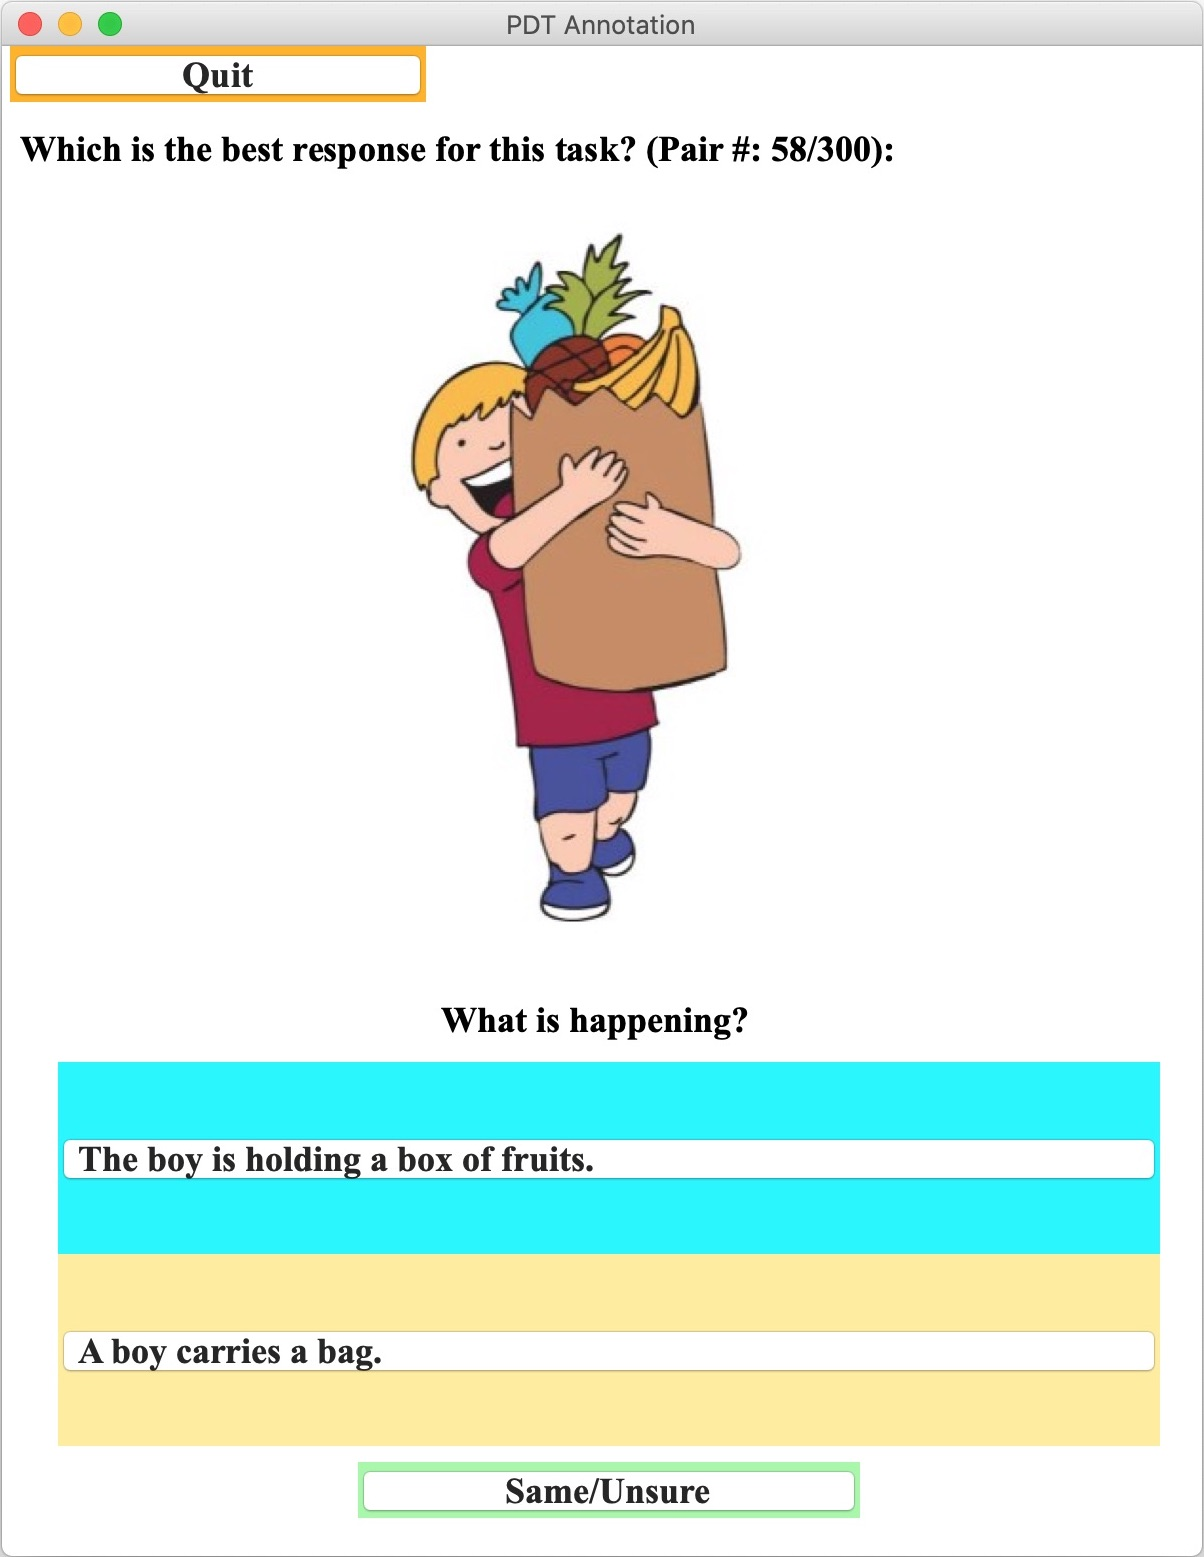
\includegraphics[width=0.85\columnwidth]{figures/ab_interface.jpg} \\
\end{tabular}
\caption{\label{fig:preference-interface} Annotation interface used for the preference test.}
\end{center}
\end{figure}

The preference test interface (Figure~\ref{fig:preference-interface}) was similar to that used for annotating the features. For each preference decision, a pair of responses along with the item image and question were presented to the annotator. The annotations for the responses were not included, but given their familiarity with the feature annotation, the annotators could probably determine the value for each feature if they tried.

Example response pairs and decisions are shown in Table~\ref{tab:preference-example-pairs}. For the first pair, both annotators preferred \textit{The boy is carrying groceries} over \textit{The boy carries the bag}. While the annotation features were not directly used during the preference test, we can infer here that the present progressive \textit{is carrying} was preferable to the simple present \textit{carries}, and indeed it more directly answers the question \textit{What is happening?} and thus better satisfies the \feat{answerhood} feature. The use of the more descriptive \textit{groceries} over \textit{bag} also likely contributed to the preference, and arguably this better satisfies the \feat{core event} feature.

\begin{table}[htb!]
\begin{center}
\begin{tabular}{|l|l|l|l|}
\hline
 Response & A1 & A2 & Agree \\
\hline
\hline
A: The boy carries the bag. & \multirow{2}{*}{B} & \multirow{2}{*}{B} & \multirow{2}{*}{yes} \\
\cline{1-1}
B: The boy is carrying groceries. & & & \\
\hline
\hline
A: The boy is holding a box of fruits. & \multirow{2}{*}{B} & \multirow{2}{*}{Same} & \multirow{2}{*}{no} \\
\cline{1-1}
B: A boy carries a bag. & & & \\
\hline
\hline
A: Little boy Towing the grocery to the car & \multirow{2}{*}{A} & \multirow{2}{*}{B} & \multirow{2}{*}{no} \\
\cline{1-1}
B: The boy is excited about his bag of groceries. & & & \\
\hline
\end{tabular}
\caption{\label{tab:preference-example-pairs} Preference test sample responses pairs, annotator decisions (\textit{A1} \& \textit{A2}) and agreement for the item shown in Figure~\ref{fig:preference-interface}.}
\end{center}
\end{table}
%\lk{add annotation vectors to table}

For the two disagreements shown in the table, one could make a reasonable argument for preferring either response (or marking them \textit{same} in quality); this is true for  most of the 35 disagreements in the sample. Disagreement over \textit{The boy is holding a box of fruits} and \textit{A boy carries a bag} seemed to involve the weighing of issues related to \feat{answerhood} (\textit{\textbf{is} hold\textbf{ing}} versus \textit{carries}), \feat{core event} (i.e., the descriptiveness of \textit{a box of fruits} versus \textit{a bag}) and \feat{verifiability} (with \textit{box} being quite clearly inaccurate). The disagreement in the third pair involved similar \feat{answerhood} issues as well as potential concerns related to \feat{grammaticality} (e.g., response A is a sentence fragment and contains a bare noun). Moreover, \textit{is excited about} in response B would likely not satisfy the \feat{core event} feature, while in response A, \textit{towing} is a questionable verb choice, and \textit{to the car} would arguably violate \feat{verifiability} because the image contains no car.

Agreement was calculated for the 300 response pairs judged by both annotators, presented in Table~\ref{tab:preference-agreement}. The agreement rate of 0.883 with a Cohen's kappa of 0.692 confirmed that high agreement on this task is both possible and reliable \citep{landis1977measurement, artstein:massimo:2008}. Moreover, the disagreements appeared to be noise spread among all features, rather than an indication of difficulty with a particular feature. With these scores, I was confident in using the full set of Annotator 1's 1,200 A/B decisions to derive the feature weights.

\begin{table}[htb!]
\begin{center}
\begin{tabular}{|l|l|l|}
\hline
 Chance Agree & Observed Agree & Kappa \\
\hline
0.621 & 0.883 (265/300) & 0.692 \\
\hline
\end{tabular}
\caption{\label{tab:preference-agreement} Preference test agreement scores for two annotators on a sample of 300 responses pairs, showing chance agreement, observed agreement and Cohen's Kappa.}
\end{center}
\end{table}

To calculate the weights, the total number of times a feature occurred with the dispreferred response in a test pair was subtracted from the total number of times that feature occurred with the preferred response to yield the net count for that feature. 87 pairs ruled \textit{same} (no preference) were omitted. The net counts of all five features were summed. The net count for each feature was then divided by this total net sum to yield the weight---this represents the degree to which each feature contributes to a response's perceived quality. The sum of the weights is 1.0. The counts and weights are shown in Table~\ref{tab:feature-weights}.

\begin{table*}[htb!]
\begin{center}
\begin{tabular}{|l||l|l|l|l|l|l|}
\hline
	& \feat{Core} & \feat{Answer} & \feat{Gramm} & \feat{Interp} & \feat{Verif} & Total \\
\hline
\hline
Tot. Pref. & 944 & 807 & 910 & 1021 & 1026 & 4708 \\
\hline
Tot. Dispref. & 367 & 660 & 822 & 667 & 611 & 3127 \\
\hline
\hline
Net Pref. & 577 & 147 & 88 & 354 & 415 & 1581 \\ 
\hline
\hline
Weight & 0.365 & 0.093 & 0.056 & 0.224 & 0.263 & 1.0 \\
\hline
\end{tabular}
\caption{\label{tab:feature-weights} Annotation counts and weights for each feature, based on a sample of 1,200 response pairs (of which 87 pairs were marked ``same'' and thus omitted). \textit{Tot. Pref.} \& \textit{Tot. Dispref.} are the number of times the feature occurred with the preferred or dispreferred response. Each weight is the feature's net preferred count divided by the total net preferred count (for all five features) of 1581.}
\end{center}
\end{table*}

The weights yielded from the preference test are well aligned with my intuitions about the features and their importance in the PDT and seem to support this work's ethos of content and communication over form. The features that relate closely to meaning carry the most weight. \feat{Core event}, which directly addresses the focus of the image, ranks well above the other features in terms of weight. \feat{Verifiability}, which limits the scope of response content, and \feat{interpretability}, which addresses a response's ability to communicate content, have similar weights that indicate a medium degree of importance. Finally, \feat{answerhood}, which deals with discourse and pragmatics, and \feat{grammaticality}, which only addresses surface forms, carry much lesser weights, as expected.

\section{Holistic Scoring and Ranking}
\label{sec:holistic-scoring}
The feature weights established by the preference tests were applied to the binary annotations to produce a holistic score for each response, which I call the \textbf{weighted annotation score}.

\begin{table}[htb!]
%Weight & 0.365 & 0.093 & 0.056 & 0.224 & 0.263 & 1.0 \\
\begin{center}
%\begin{tabular}{|p{3.7cm}|c|c|c|c|c|}
\begin{tabular}{|l||r|r|r|r|r||r|r|}
\hline
\textit{What is happening?} & C & A & G & I & V & WAS & WAR \\
\hline
\hline
Child is eating pizza. & 0.365 & 0.093 & 0.000 & 0.224 & 0.263 & 0.945 & 1 \\
\hline
Tommy is eating pizza. & 0.365 & 0.093 & 0.056 & 0.224 & 0.000 & 0.738 & 2 \\
\hline
The boy's eating his fav... & 0.000 & 0.093 & 0.056 & 0.000 & 0.000 & 0.514 & 3 \\
\hline
Pizza is this boy's fav... & 0.000 & 0.000 & 0.056 & 0.000 & 0.000 & 0.056 & 4 \\
\hline
\end{tabular}
\caption{\label{tab:applied-weights} Example NNS responses (see Table~\ref{tab:dev-transitive}) with feature weights applied to the binary annotations, resulting in weighted annotation scores (\textit{WAS}) and a weighted annotation ranking (\textit{WAR}).}
\end{center}
\end{table}

%or S$_{WA}$. 
For each item, I ranked the NNS responses according to this score. I call the resulting ranking a \textbf{weighted annotation ranking}. A toy example of such a ranking is presented in Table~\ref{tab:applied-weights}, where the binary annotations have been multiplied by their weights. In the first row, for example, we see that a ``1'' for \feat{core event} has been multiplied by the weight for \feat{core event} (1 $\times$ 0.365 $=$ 0.365), and a ``0'' for \feat{grammaticality} has also been multiplied by the weight for \feat{grammaticality} (0 $\times$ 0.056 $=$ 0.000). Because these rankings are based on human annotator decisions, they can serve as a benchmark for comparing the output of an automatic scoring system, as discussed in Chapter~\ref{chap:optimization}.

The NS responses were also annotated for the binary features, but in the current work there is no practical use for a weighted annotation ranking of the NS responses. However, by applying the weights and obtaining weighted annotation scores for the NS responses, I can compare the holistic performance of NS and NNS participants. As shown in Table~\ref{tab:was1}, in terms of weighted annotation scores, \textit{familiar native speakers} (\textit{FNSs}; see Section~\ref{sec:participants}) outperformed NNSs, who outperformed \textit{crowdsourced native speakers} (\textit{CNSs}). The FNSs had the highest rate of perfect responses, the lowest rate of zero-scoring responses and the highest mean weighted annotation scores. Moreover, the standard deviation shows that FNSs had the least varied weighted annotation scores, which makes sense as scores for this group were heavily skewed toward the upper limit. In each of these measures, the FNSs were followed by the NNSs, then the CNSs. It should be noted that these scores cover the entire set of all responses for all items, which includes the two responses from NSs per item, whereas the NNSs provided only a single response per item.


\begin{table*}[htb!]
\begin{center}
\begin{tabular}{|l||r||r|r||r|}
\hline
 & NNS	& CNS & FNS & C$+$F \\
\hline
\hline
Total & 4230 & 7723 & 1580 & 9303 \\
\hline
\hline
Perfect & 0.614 & 0.495 & 0.692 & 0.528 \\
\hline
Zero & 0.011 & 0.048 & 0.001 & 0.040 \\
\hline
\hline
Mean & 0.862 & 0.763 & 0.880 & 0.783 \\
\hline
Median & 1.000 & 0.944 & 1.000 & 1.000 \\
\hline
Std Dev & 0.248 & 0.323 & 0.226 & 0.312 \\
\hline
\end{tabular}
\caption{\label{tab:was1} Comparing scores for non-native speakers (\textit{NNS}), \textbf{crowdsourced} native speakers (\textit{CNS}) and \textbf{familiar} native speakers (\textit{FNS}) across all items. \textit{C$+$F} is the combination of CNS and FNS (i.e., \textit{all} NS). \textit{Total} is the response count. \textit{Perfect} and \textit{Zero} are the rates of responses with weighted annotation scores of 1.0 and 0.0, respectively. The \textit{Mean}, \textit{Median} and \textit{Standard Deviation} values here are weighted annotation scores.}
\end{center}
\end{table*}

The relative performance of these three groups has important implications for how this data is used and how data for related purposes might be collected in the future. Because my work is geared toward communicative ICALL rather than grammatical error correction or placement testing, the models I use must be flexible enough to process NNS responses without heavily penalizing them for minor issues in form or usage. For my purposes, models built only from FNS responses would be overfitted to the near-perfect language usage of the FNS group. Models built from the more varied CNS responses are preferable for my purposes. In effect, they will allow for more of the variations in form and usage that we see among the NNS responses. In other words, an FNS-based model will identify those responses that closely match a limited set of well-formed possibilities, but it will harshly penalize other variations, resulting in scores that tend toward the high and low ranges. A CNS-based model will be less strict; slight deviations from NS usage will be penalized less harshly, and scores will be distributed more evenly across the range from 0.0 to 1.0.

Due to the sparsity of the FNS data, it was not possible to analyze it on a more granular level. With more data from the CNS group, however, it was possible to break down the CNS metrics seen in Table~\ref{tab:was1} for a closer look, as shown in Table~\ref{tab:was2}.

The trends seen in the CNS table confirmed my intuitions about the data---scores decrease as complexity and variation increase. First response scores were higher than second response scores. This makes sense given my observations from Chapter~\ref{chap:data}, where I found a higher rate of bad faith or low-effort answers among the second responses, likely owing to fatigue and boredom, and a higher type-to-token ratio, indicating a higher rate of unique responses (see Table~\ref{tab:ttr1v2}). This increase in variation means more creative responses, which are more likely to include unverifiable details, for example. Similarly, untargeted response scores were lower than targeted response scores. This can also be explained by the greater degree of variability among untargeted responses, as discussed in Chapter~\ref{chap:data} (see Tables~\ref{tab:ttr},~\ref{tab:ttr1v2} and~\ref{tab:ttr1v1}). This is expected, because the subject is provided in targeted prompts but not untargeted prompts, so naturally the untargeted responses included more cases where the subject is incorrect, irrelevant or unclear. Finally, among the item (verb transitivity) types shown in Table~\ref{tab:was2}, the scores decreased as the complexity increased; intransitive scores were highest, followed by transitives and then ditransitives. Again, this correlates with type-to-token ratios (see Tables~\ref{tab:ttr},~\ref{tab:ttr1v2} and~\ref{tab:ttr1v1}). 

\begin{table*}[htb!]
\begin{center}
\begin{tabular}{|l||r|r||r|r||r|r|r|}
\hline
 & R1 & R2 & Target & Untarg & Intran & Trans & Ditran \\
\hline
\hline
Total & 3872 & 3851 & 3877 & 3846 & 2592 & 2569 & 2562 \\
\hline
\hline
Perfect & 0.623 & 0.366 & 0.535 & 0.454 & 0.519 & 0.502 & 0.463 \\
\hline
Zero  & 0.037 & 0.058 & 0.043 & 0.053 & 0.040 & 0.051 & 0.053  \\
\hline
\hline
Mean  & 0.838 & 0.687 & 0.772 & 0.753 & 0.775 & 0.757 & 0.756  \\
\hline
Median  & 1.000 & 0.851 & 1.000 & 0.944 & 1.000 & 1.000 & 0.907  \\
\hline
Std Dev  & 0.286 & 0.340 & 0.315 & 0.330 & 0.319 & 0.330 & 0.320  \\
\hline
\end{tabular}
\caption{\label{tab:was2} Examining \textbf{crowdsourced} native speaker response scores in different contexts: first and second responses (\textit{R1} and \textit{R2});  targeted and untargeted prompts; intransitives, transitives, and ditransitives. (See Table~\ref{tab:was1}.)}
\end{center}
\end{table*}

These observations strengthened my conviction that CNS-based scoring models are preferable for my approach, while higher-quality, more uniform FNS-based scoring models would be preferable for stricter contexts like language assessment or placement testing. Naturally, the best way to score NNS responses would be to use models trained on NNS responses. However, these responses would need to be validated or classified in some way by annotators, which would require developing new annotation guidelines. The idea is also counter to the motivations behind my work, because it means every new item would require manual annotation of NNS responses by experts in order to train a scoring model, which places a greater burden on educators or researchers who might follow this approach. Ideally, a system could train an initial model based on unannotated CNS responses; after scoring some NNS responses, it could then add examples of the highest scoring NNS responses to the training data and retrain iteratively---an approach known as self-training. I do not explore the use of NNS responses as training data, but future work to do so can build on the work here.




\section{Annotation Conclusions}
\label{sec:annotation-conclusions}

%\subsection{Annotator feedback}
The SAILS corpus presented here was developed with specific research in mind, but also in the hopes that it may be used to address a broad range of questions. I have demonstrated here a set of binary features that were successfully implemented with reliable levels of inter-annotator agreement. These features were defined with an eye toward content analysis and ICALL, but the annotations and raw responses would also be useful for question answering, dialog systems, pragmatics modeling, visual references and other challenges in natural language processing. The feature set can also be expanded to better suit other purposes, and the task can easily be extended to include new items. To facilitate expansion, guidelines, task materials and annotation tools are included with the corpus.\footnote{https://github.com/sailscorpus/sails}

%\smallskip
A number of lessons have been learned in this process, and as I intend this work to be extendable, a few suggestions are in order. The inclusion of any symbols or numerals in items should be avoided as they resulted in response complications; some participants gave clever ``meta'' responses (\textit{She's breathing in music notes}, rather than \textit{She's singing}), and others focused on the symbols rather than the abstract concepts they represent (\textit{The teacher is teaching `2 $+$ 2 $=$ 4'}, rather than \textit{The teacher is teaching math}). The comparison of crowdsourced NS data with the data of familiar NS participants and the NNS student data made it clear that motivations and task environment can affect the quality of responses.
%, and these factors must be considered during data collection.

%\smallskip
%The current work is appropriate for a broad examination of variation; if one has more specific research questions in mind, however, a more tailored approach to this kind of data collection and annotation would likely mean more efficiency in terms of effort and expense. 
Additionally, more clearly defining acceptable core events could lessen the ambiguity for annotators. While I intend the NS responses collected here to be useful for comparing with NNS responses and addressing related research questions, for specific applications like language testing, the use of expert annotators and constructed reference materials or models may be more desirable or cost effective (see, for example, \citet{somasundaran:chodorow:14}).
